\section{Methodology}
\label{section:algorithm}

\textbf{High-level idea.} We assemble a post-generation verification layer \emph{entirely
from published techniques} and evaluate it on the course-provided RAG system (Program~1
builds the vector DB; Program~2 retrieves and generates cited answers). The pipeline:
(0)~\emph{Language detection (course HW1)}: a character-level language-identification model
(from course HW1) tags the language of each claim and cited passage, so cross-lingual /
code-switched pairs---common in the Chinese corpus and harder to verify---can be handled
separately.
(1)~\emph{Claim segmentation}: split the answer into atomic, verifiable claims using
published extraction (e.g., VeriScore~\citep{song2024veriscore}) or simple heuristics.
(2)~\emph{Citation alignment}: bind each claim to the text of the document(s) it cites.
(3)~\emph{Grounding scoring}: score each claim against its cited passage with the
\emph{published scorers under comparison}---embedding-similarity, NLI entailment
(TRUE~\citep{honovich2022true}), LLM-as-judge (RAGAS~\citep{es2024ragas}), and
sampling consistency (SelfCheckGPT~\citep{manakul2023selfcheckgpt}).
(4)~\emph{Decision}: apply each scorer's documented decision rule to label claims as
supported / uncertain / unsupported.

This is an \emph{evaluation and application} study: the research question is which
published verification technique(s) transfer well to a RAG QA system and at what
accuracy/cost/reproducibility trade-off. We contribute the comparison and the adoption
recommendation, not a new scoring method.

\begin{figure}[h]
\centering
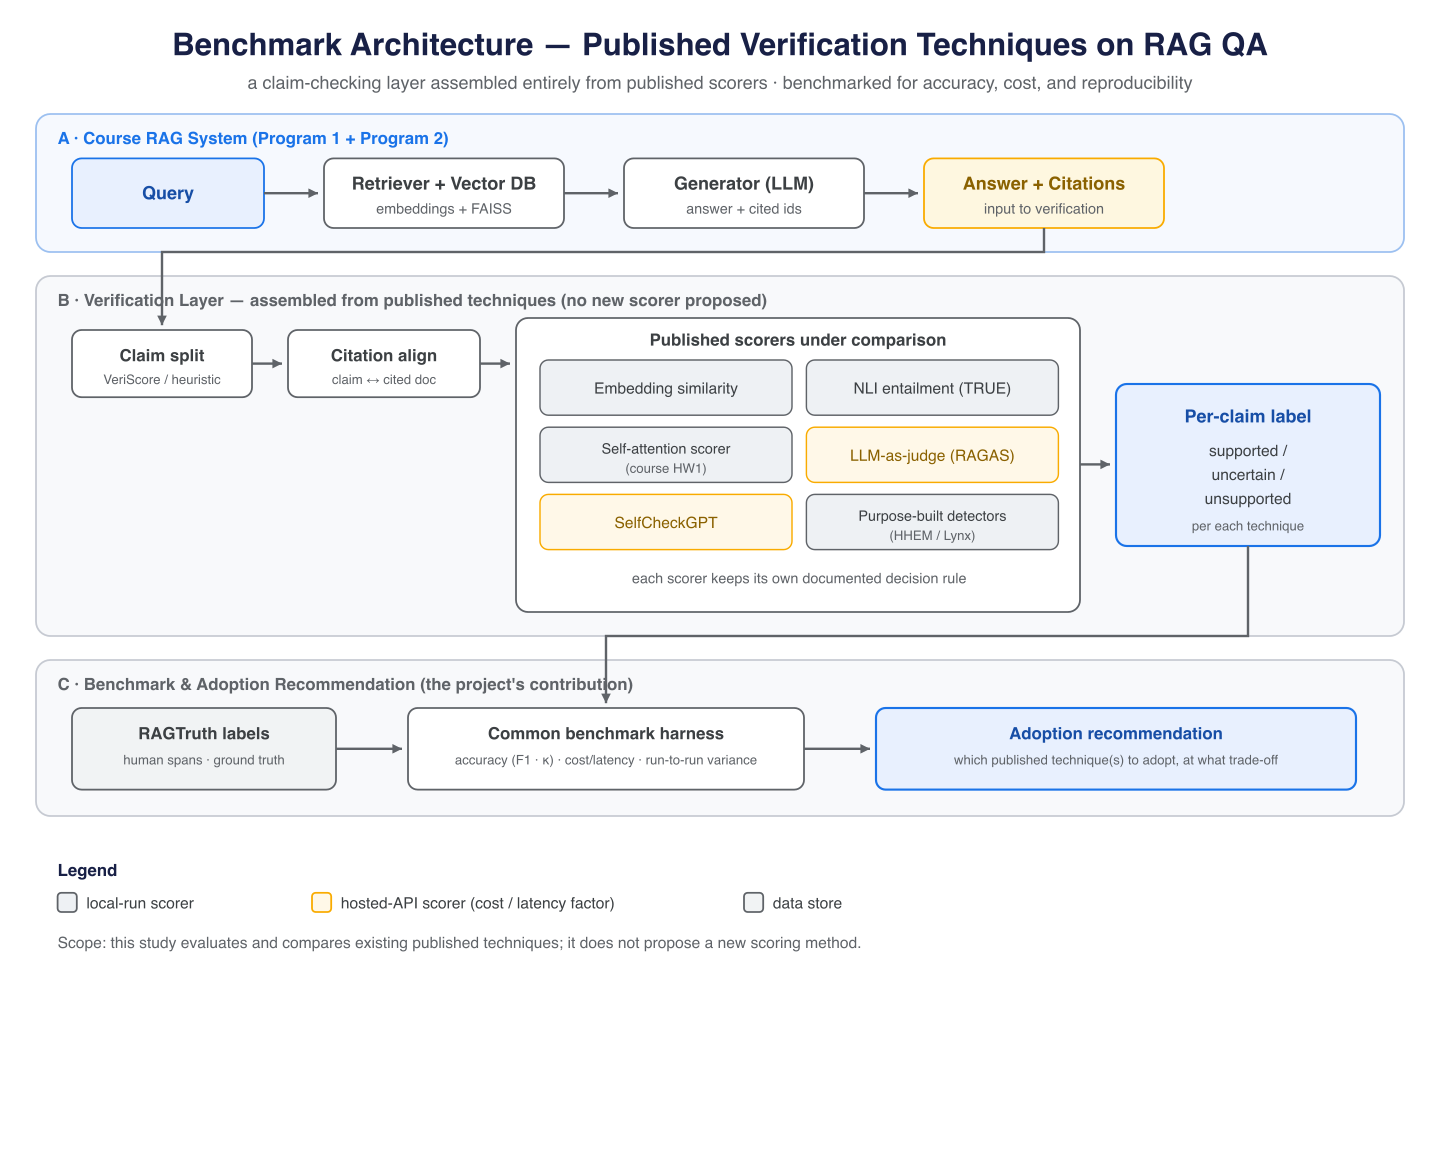
\includegraphics[width=\textwidth]{figures/bench-arch.png}
\caption{Benchmark architecture. A claim-checking layer (zone~B) assembled entirely from
published scorers is run on the course RAG system (zone~A); every technique keeps its own
documented decision rule and is scored by a common benchmark harness against RAGTruth human
labels (zone~C). The project's contribution is the comparison and the adoption
recommendation, not a new scoring method.}
\label{fig:layer}
\end{figure}
